\documentclass[a4paper]{article}
\usepackage[utf8]{inputenc}
\usepackage[spanish, es-tabla]{babel}

\usepackage{amsmath}
\usepackage{amsfonts}
\usepackage{amssymb}

\usepackage{float}
\usepackage{graphicx}
\usepackage{subcaption}
\captionsetup{compatibility=false}

\usepackage{multirow}
\setlength{\doublerulesep}{\arrayrulewidth}

\usepackage{array}
\newcolumntype{C}[1]{>{\centering\let\newline\\\arraybackslash\hspace{0pt}}m{#1}}

\usepackage[american]{circuitikz}

\usepackage{fancyhdr}

\usepackage{units} 

\pagestyle{fancy}
\fancyhf{}
\lhead{22.01 Teoría de Circuitos}
\rhead{Mechoulam, Lambertucci, Rodriguez, Londero}
\rfoot{Página \thepage}
\begin{document}

\section{Introducción a diseño de filtros.}
%%%%%%%%%%%%%%%%%%%%%%%%%%%%%%%%%%%
\subsection{Introducción.}
El \textbf{Gyrator} es un componente electrónico inicialmente propuesto como el quinto componente lineal y pasivo luego del resistor, capacitor, inductor y transformador ideal, teninedo la propuesto en 1948 por Bernard D. H. Tellegen el componente podría ... siendo caracterizado por un cuadripolo con parametros impedancia:
$$ Z= \left(\begin{matrix}0&-R\\R&0\end{matrix}\right) $$
Donde R sería la resistencia interna del Gyrator.

\begin{figure}[H]	
	\centering
	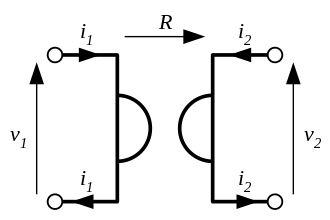
\includegraphics[width=0.7\textwidth]{gyratorsimb.png}
	\caption{Simbolo eléctrico del Gyrator.}
	\label{fig:gyrsimb}
\end{figure}
Realmente es implementado utilizando opamps, y uno de los usos mas populares es para la inversión de impedancias, permitiendo simular un inductor utilizando otros componentes.La configuración generalmente utilizada es la siguiente:
\begin{figure}[H]	
	\centering
	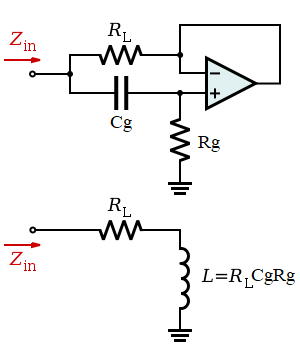
\includegraphics[width=0.5\textwidth]{gyrop.png}
	\caption{Equivalente del circuito Gyrator.}
	\label{fig:gyrop}
\end{figure}

%%%%%%%%%%%%%%%%%%%%%%%%%%%%%%%%%%%%%%%%%
\subsection{Calculo analítico.}
Utilizando el circuito de la figura (\ref{fig:gyrop}) se plantearon las siguientes ecuaciones:
\begin{align}   V_{Out} = V^- \label{eq:1}\end{align}
\begin{align} V_{Out} = A(s) \cdot (V^+-V^-)\label{eq:2}\end{align}
\begin{align} A(s)= \frac{A_0}{1+\frac{s}{\omega'}}\end{align}
\begin{align} I_{In}=\frac{V_{In}-V^-}{R_L}+\frac{V^+}{R_g}\end{align}
\begin{align} V^+=V_{In}\cdot \frac{R_g}{R_g+\frac{1}{sC_g}} \end{align}
primero observaremos que en utilizando (\ref{eq:1}) y (\ref{eq:2}) se llega a que 
\begin{align}V^- =V^+ \cdot \frac{A(s)}{A(s)+1} = V^+ \cdot \frac{A_0}{A_0+1+\frac{s}{\omega'}} \approx V^+ \cdot \frac{1}{1+\frac{s}{GBP}}   \end{align}
Donde GBP es un parámetro propio del operacional y suele ser del orden de los MHz. Por lo tanto este termino sería desprecianle siempre que el rango de frecuencias en los cuales se trabaje sea menor a... \center \textcolor{red}{Obtener algun valor significativo}
, teniendo en cuenta esa aproximacion se pueden llegar a las siguientes expresiones:
\begin{align}H(s)= \frac{R_g}{R_g+\frac{1}{sC_g}} \end{align}


\begin{align}Z_{In}=\frac{R_LR_gC_gs+R_L}{sC_gR_L+1}\underset{C_gR_gR_Ls << 1}{\approx}R_gC_gR_L \cdot s + R_g \end{align}

Bajo estos supuestos se puede considerar la impedancia de entrada como una bobina con $L=R_gC_gR_L $ y $R_g$ siendo esta R la parte resistiva de la inductancia.
\subsubsection{Gyrator vs Inductor}

\subsubsection{Impedancia de entrada.}

\subsubsection{Elección operacional.}

%%%%%%%%%%%%%%%%%%%%%%%%%%%%%%%%%%%%%%
 \flushleft
\subsection{Filtros de segundo orden.}
Los filtros a implemetar en este trabajo serán filtros de segundo orden siendo estos Low-Pass, High-Pass, Band-Pass y Band-Reject. Y tendran las siguientes especificaciones de diseño:
\begin{table}[H]
\begin{center}
\begin{tabular}{|c|c|c|c|}
\hline
\textbf{Tipo de Filtro} & \textbf{$f_p$ [Hz]} & \textbf{$f_a$ [Hz]} & \textbf{$f_c$ [Hz]} \\ \hline
\textbf{LP}             & 1000                & 3500                & \textbf{-}          \\ \hline
\textbf{HP}             & 10500               & 3000                & \textbf{-}          \\ \hline
\textbf{BP}             & -                   & -                   & 2000                \\ \hline
\textbf{BR}             & -                   & -                   & 3000                \\ \hline
\end{tabular}
\caption{Tabla de especificaciones.}
\label{tab:specs}
\end{center}
\end{table}
Para el caso de LP que tenga ganancia unitaria para la continua que tenga una ganancia mayor a -3dB para frecuencias menores a $f_p$ y menor a -10dB para frecuencais mayores a $f_a$. Para el HP se desea que tenga ganancia unitaria para valores de $f$ muy grandes, que tenga una ganancia mayor a -3dB para frecuencias mayores a $f_p$ y menor a -10dB para frecuencais menores a $f_a$
Algunos parametros que vale la pena recordar de filtros de segundo orden son:
\begin{table}[H]
\begin{center}
\begin{tabular}{c|cl}
$\omega_0$: & Frecuencia de corte del sistema en [$\frac{rad}{s}$] & =$\frac{1}{\sqrt{LC}}$         \\
$\xi$:      & Factor de Amortiguamiento del sistema.               & =$\frac{R\sqrt{C}}{2\sqrt{L}}$ \\
Q:          & Selectividad del sistema                             & =$\frac{1}{2\xi}$             
\end{tabular}
\end{center}
\caption{Parametros útiles.}
\label{tab:utils}
\end{table}

%%%%%%%%%%%%%%%%%%%%%%%%%%%%%%%%%%%%%%%%%%%%
\subsection{High Pass.}
\subsubsection{Circuito utilizando inductor.}
El circuito propuesto para realizar un filtro pasa altos clasicamente es el siguiente:
\begin{figure}[H]	
	\centering
	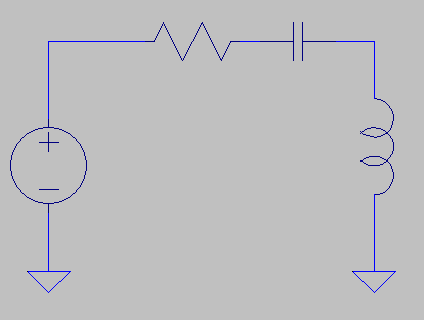
\includegraphics[width=0.7\textwidth]{basicHP.PNG}
	\caption{Filtro High-Pass básico.}
	\label{fig:basHP}
\end{figure}
Para este circuito es sumamente facil obtener la transferencia, basta con plantear un divisor resistivo, con lo cual se llega a:
\begin{align} 
H(s)=\frac{s^2LC}{s^2LC+sRC+1}
 \end{align}

\subsubsection{Circuito utilizando Gyrator.}
Para la implementación de este filtro utilizando un Gyrator dado a que este usualmente esta referenciado a tierra  se optó por el siguiente diseño:
\begin{figure}[H]	
	\centering
	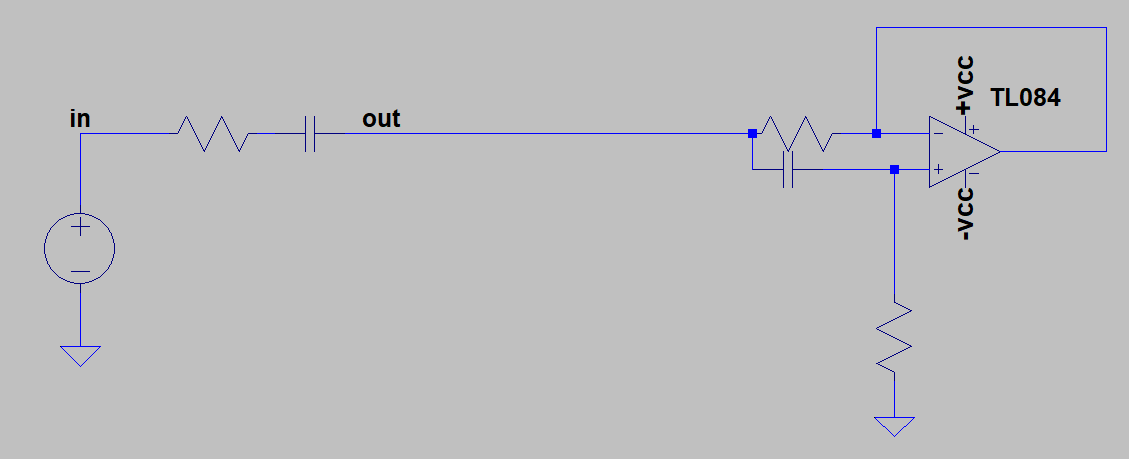
\includegraphics[width=0.7\textwidth]{gyrHP.PNG}
	\caption{Filtro High-Pass implementado con Gyrator.}
	\label{fig:gyrHP}
\end{figure}
\subsubsection{Comparación de modelos.}
\subsubsection{PCB.}
\subsubsection{Respuesta en frecuencia.}
\subsubsection{Analisis de resultados.}

\newpage
%%%%%%%%%%%%%%%%%%%%%%%%%%%%%%%%%%%%%%%%%%%%
\subsection{Low Pass.}
\subsubsection{Circuito utilizando inductor.}
El circuito propuesto para realizar un filtro pasa bajos clasicamente es el siguiente:
\begin{figure}[H]	
	\centering
	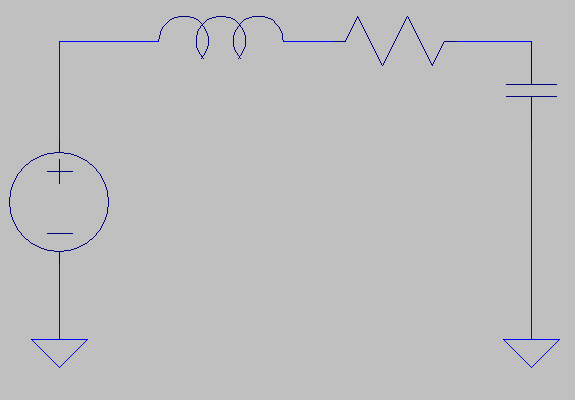
\includegraphics[width=0.7\textwidth]{basicLP.PNG}
	\caption{Filtro Low-Pass básico.}
	\label{fig:basLP}
\end{figure}

\subsubsection{Circuito utilizando Gyrator.}
\begin{figure}[H]	
	\centering
	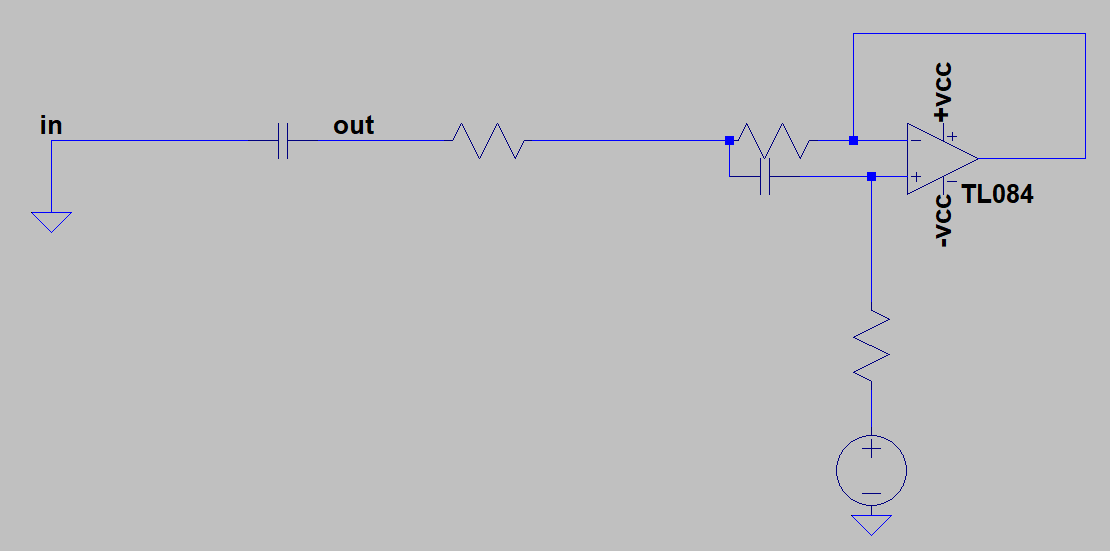
\includegraphics[width=0.7\textwidth]{gyrLP.PNG}
	\caption{Filtro Low-Pass implementado con Gyrator.}
	\label{fig:gyrLP}
\end{figure}
\begin{equation} H(s)= \frac{\left(Cg Rl s + 1\right)}{C Cg R Rl s^{2} + C Cg Rg Rl s^{2} + C R s + C Rl s + Cg Rl s + 1} \end{equation}
\subsubsection{Comparación de modelos.}
\subsubsection{PCB.}
\subsubsection{Respuesta en frecuencia.}
\subsubsection{Analisis de resultados.}
\newpage
%%%%%%%%%%%%%%%%%%%%%%%%%%%%%%%%%%%%%%%%%%%%
\subsection{Band Pass.}
\subsubsection{Circuito utilizando inductor.}
El circuito propuesto para realizar un filtro pasa banda clasicamente es el siguiente:
\begin{figure}[H]	
	\centering
	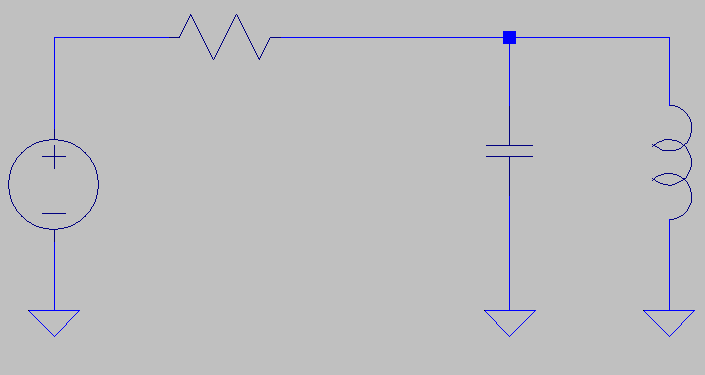
\includegraphics[width=0.7\textwidth]{basicBP.PNG}
	\caption{Filtro Band-Pass básico.}
	\label{fig:basBP}
\end{figure}

\subsubsection{Circuito utilizando Gyrator.}
\begin{figure}[H]	
	\centering
	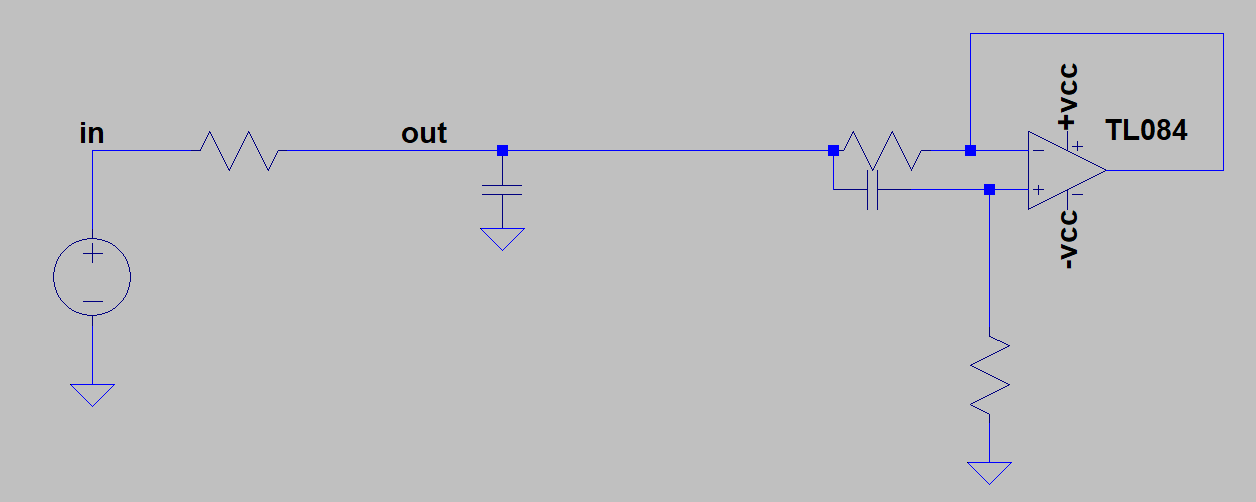
\includegraphics[width=0.7\textwidth]{gyrBP.PNG}
	\caption{Filtro Band-Pass implementado con Gyrator.}
	\label{fig:gyrBP}
\end{figure}
\subsubsection{Comparación de modelos.}
\subsubsection{PCB.}
\subsubsection{Respuesta en frecuencia.}
\subsubsection{Analisis de resultados.}
\newpage
%%%%%%%%%%%%%%%%%%%%%%%%%%%%%%%%%%%%%%%%%%%%
\subsection{Band Reject.}
\subsubsection{Circuito utilizando inductor.}
El circuito propuesto para realizar un filtro rechaza banda clasicamente es el siguiente:
\begin{figure}[H]	
	\centering
	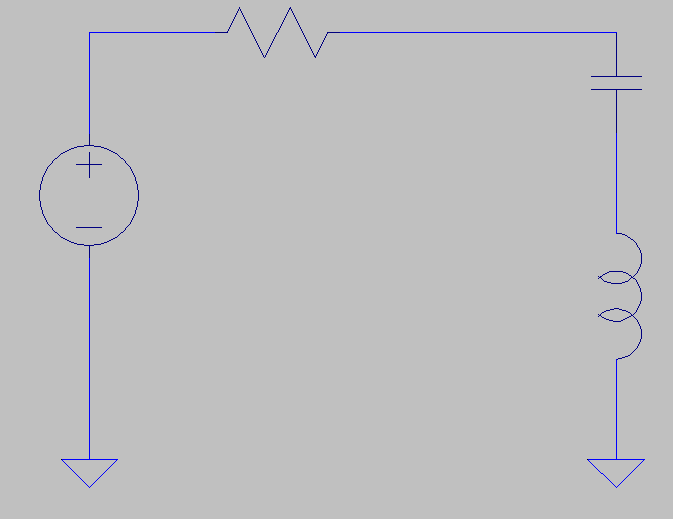
\includegraphics[width=0.7\textwidth]{basicBR.PNG}
	\caption{Filtro Band-Reject básico.}
	\label{fig:basBR}
\end{figure}
\subsubsection{Circuito utilizando Gyrator.}
\begin{figure}[H]	
	\centering
	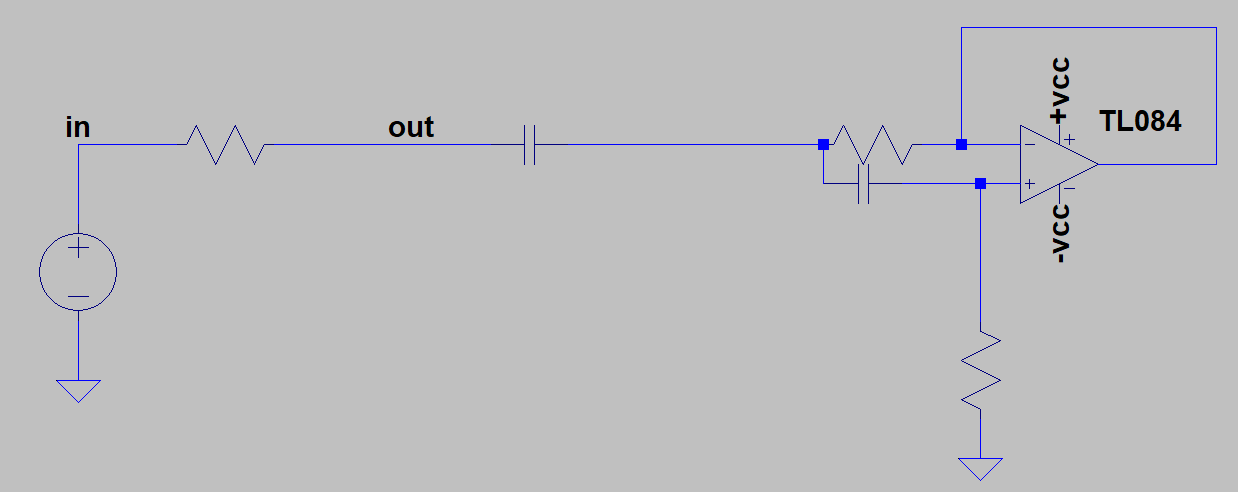
\includegraphics[width=0.7\textwidth]{gyrBR.PNG}
	\caption{Filtro Band-Reject implementado con Gyrator.}
	\label{fig:gyrBR}
\end{figure}

\subsubsection{Comparación de modelos.}
\subsubsection{PCB.}
\subsubsection{Respuesta en frecuencia.}
\subsubsection{Analisis de resultados.}

\end{document}
%\begin{align}\end{align}